\section{Cafe: Predicting Physical Attraction with Deep Learning-Based Systems}

\subsection{Introdução ao Conceito}

\textbf{Definição:} \\
O projeto ``Cafe'' é um aplicativo de namoro que utiliza aprendizado profundo, especificamente redes neurais convolucionais (CNNs), para prever a atratividade física de indivíduos. Ele utiliza técnicas de aprendizado por transferência para personalizar a experiência do usuário, sendo uma referência valiosa para aplicar CNNs na análise de preferências visuais em trabalhos de conclusão de curso \textcolor{blue}{[\cite{DesiPilla}]}.

\textbf{Contextualização:} \\
No cenário atual dos aplicativos de namoro, a aparência física é frequentemente um fator decisivo. O ``Cafe'' visa otimizar esse processo através de algoritmos de deep learning, treinando modelos para analisar imagens de perfis de maneira eficiente e automatizada.

\subsection{Desenvolvimento Teórico}

\textbf{Explicação Detalhada:}

O projeto ``Cafe'' aplica técnicas de aprendizado por transferência, utilizando a arquitetura VGGNet como base para treinar redes neurais em um conjunto de imagens coletadas do Google. A CNN analisa imagens de perfis de namoro para prever se uma foto é atraente ou não, de acordo com as preferências do autor.



\textbf{Conjunto de Dados:} \\
As imagens usadas no treinamento foram retiradas do Google, abrangendo uma variedade de etnias e idades. Foram aplicadas técnicas de aumento de dados para melhorar a diversidade e representatividade do conjunto de dados.

\textbf{Modelagem de Preferências:} \\
A abordagem se concentra em personalizar recomendações com base em preferências pessoais, utilizando rótulos de ``gostar'' ou ``não gostar'' para treinar o modelo a prever a atratividade com precisão.
\clearpage
\begin{figure}
    \centering
    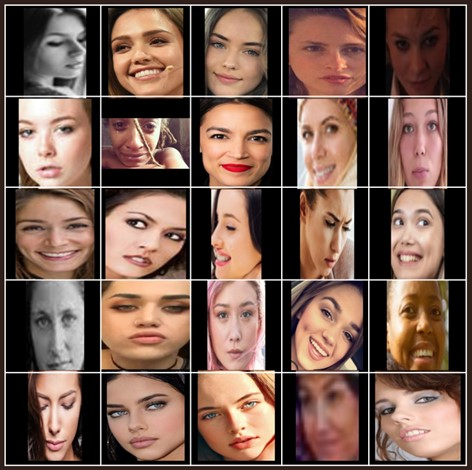
\includegraphics[width=0.8\linewidth]{faces.png}
    \caption{Exemplo de Imagens Usadas.} \protect\href{https://github.com/DesiPilla/cafe}{(\textcolor{blue}{Fonte})}
    \label{fig:cnn}
\end{figure}



\subsection{Componentes Técnicos}

\textbf{Adaptação do Algoritmo:}

\begin{itemize}
    \item \textbf{Camadas Densas:} As camadas densas finais do VGG16 são removidas e substituídas por novas camadas treináveis, otimizadas para classificar atratividade em perfis de namoro.
    \item \textbf{Transferência de Aprendizado:} A técnica de aprendizado por transferência é usada para economizar tempo computacional e melhorar a precisão, ajustando camadas pré-treinadas para o conjunto de dados específico.
\end{itemize}

\begin{itemize}
    \item \textbf{VGGNet e VGG16:} \\
    VGGNet é uma arquitetura de rede neural convolucional desenvolvida pelo Visual Geometry Group da Universidade de Oxford. Destaca-se por sua simplicidade e eficácia na classificação de imagens, utilizando camadas de convolução com filtros pequenos de 3x3, intercaladas com camadas de pooling. A VGG16 é uma variante que consiste em 16 camadas com parâmetros, incluindo 13 camadas de convolução e 3 camadas totalmente conectadas. Essa arquitetura é conhecida por sua profundidade e capacidade de aprender representações complexas de imagens \textcolor{blue}{[\cite{Simonyan2014}]}.

    \item \textbf{Aprendizado por Transferência:} \\
    O aprendizado por transferência é uma técnica que permite utilizar modelos previamente treinados, como o VGG16, para novas tarefas. Isso é feito ajustando as camadas finais do modelo para o novo conjunto de dados, economizando tempo e recursos computacionais ao aproveitar o conhecimento previamente adquirido pelo modelo \textcolor{blue}{[\cite{Krizhevsky2012}]}.

    \item \textbf{Explicabilidade (LRP):} \\
    O projeto também explora a explicabilidade dos modelos, utilizando técnicas como a Propagação de Relevância em Camadas (LRP). A LRP é uma técnica que ajuda a entender como as decisões são tomadas pela rede neural, identificando quais características de uma imagem são mais relevantes para as previsões do modelo. Isso é feito rastreando a contribuição de cada pixel na imagem original para a decisão final da rede, oferecendo uma visualização clara das áreas que mais influenciam as decisões do modelo \textcolor{blue}{[\cite{Bach2015}]}.
\end{itemize}

O ``Cafe'' demonstra o potencial de aplicar deep learning em aplicativos de namoro, otimizando o processo de recomendação com base em atratividade visual e preferências pessoais.

\section{Dataset OkCupid e Instagram Graph API}

\subsection{Utilização do Dataset OkCupid}

\textbf{Definição:} \\
O dataset OkCupid Profiles disponível no Kaggle é uma coleção rica de perfis de usuários da plataforma de encontros OkCupid. Ele inclui dados demográficos e preferências pessoais, como idade, gênero, localização, interesses e auto-descrições, tornando-o um recurso valioso para análises de comportamento e perfilagem de usuários \textcolor{blue}{[\cite{OkCupidProfiles}]}.

\textbf{Contextualização:} \\
Esses dados podem ser usados para implementar "Personality Aggregation" em sistemas de recomendação, identificando características comuns entre usuários e melhorando a personalização das recomendações. Por exemplo, informações textuais podem ser processadas usando técnicas de processamento de linguagem natural (NLP) para extrair insights sobre preferências pessoais e traços de personalidade.

\subsection{Integração com a API do Instagram Graph}

\textbf{Definição:} \\
A API do Instagram Graph é uma ferramenta que permite acessar dados de interações sociais e conexões entre usuários no Instagram. Com ela, é possível obter informações sobre quem um usuário segue, quem os segue, além de suas interações, como curtidas e comentários \textcolor{blue}{[\cite{InstagramGraphAPI}]}.

\textbf{Contextualização:} \\
Utilizando a API do Instagram Graph, pode-se modelar o grafo social de usuários, capturando as influências sociais que afetam as preferências de cada um. Este tipo de "Social Aggregation" é fundamental para compreender como as redes sociais influenciam comportamentos e escolhas, possibilitando recomendações mais precisas e baseadas em interações sociais reais.

\section{GraphRecWWW19}

\subsection{Introdução ao Conceito}

\textbf{Definição:}  
GraphRec é uma arquitetura de rede neural desenvolvida para recomendações sociais, utilizando redes neurais de grafos (GNNs). Essa abordagem integra informações de nós e a estrutura topológica de dados de grafo a alguns mecanismos presentes nos transformers, permitindo modelar de forma eficaz tanto as interações quanto as opiniões no grafo de usuário-item e no grafo social de usuário-usuário.\textcolor{blue}{[\cite{GraphRecWWW19}]}.
\textbf{Contextualização:}  
Em sistemas de recomendação social, os dados são frequentemente representados como grafos, onde nós representam usuários ou itens e as arestas representam interações ou relações sociais. GraphRec se destaca por sua capacidade de capturar e modelar essas relações complexas, combinando informações de diferentes tipos de grafos para melhorar a precisão das recomendações.

\subsection{Desenvolvimento Teórico}

\textbf{Explicação Detalhada:}

GraphRec utiliza uma combinação de técnicas de Graph Neural Networks (GNNs) e atenção para modelar dois tipos principais de grafos: o grafo usuário-item e o grafo social usuário-usuário. Esses componentes trabalham em conjunto para melhorar a capacidade do sistema de recomendação ao integrar múltiplas fontes de informação.

\begin{itemize}
    \item \textbf{Grafo Usuário-Item:}  
    Neste grafo, as arestas representam interações entre usuários e itens, muitas vezes acompanhadas de opiniões ou avaliações. O modelo utiliza agregações de itens para capturar preferências dos usuários com base nas interações passadas.

    \item \textbf{Grafo Social Usuário-Usuário:}  
    Este grafo modela as relações sociais entre usuários. A agregação social permite que o modelo entenda a influência social e como as relações entre usuários podem impactar suas preferências.

    \item \textbf{Integração com Mecanismo de Atenção:}  
    GraphRec aplica mecanismos de atenção para dar pesos diferentes a diferentes conexões no grafo, permitindo uma modelagem mais precisa das relações complexas entre nós.
\end{itemize}

\clearpage
\begin{figure}
    \centering
    \vspace{-2cm}
    \hspace*{-2.5cm} % Ajuste o valor em centímetros conforme necessário
    \includegraphics[width=1.3\linewidth]{modelo.png}
    \caption{Modelo do GraphRechWWW19} \protect\href{https://github.com/wenqifan03/GraphRec-WWW19}{(\textcolor{blue}{Fonte})}
    \label{fig:cnn}
\end{figure}

\subsection{Componentes Técnicos}

\textbf{Adaptação do Algoritmo:}

\begin{itemize}
    \item \textbf{Item Aggregation to Personality Aggregation:}  
    Nesta adaptação, o componente de agregação de itens pode ser alterado para agregar traços de personalidade, considerando traços de personalidade como itens para identificar preferências comuns entre usuários.

    \item \textbf{Social Aggregation:}  
    Este componente permanece inalterado, continuando a capturar influências sociais baseadas nas conexões entre usuários no grafo social.

    \item \textbf{Adição de Visual Aggregation:}  
    Um novo componente de agregação visual pode ser introduzido, onde Redes Neurais Convolucionais (CNNs) são usadas para extrair características visuais das imagens dos usuários, analisando aquelas que recebem likes e dislikes.
\end{itemize}

Com essas adaptações, GraphRec pode ser ajustado para analisar não apenas preferências de item, mas também traços de personalidade e preferências visuais, tornando o sistema de recomendação mais abrangente e personalizado para aplicativos de namoro.



